\documentclass{beamer}
\usepackage{beamerthemesplit}

%Definieren uns farbigen Quellcode
\usepackage{color}
\definecolor{dkgreen}{rgb}{0,0.6,0}
\definecolor{gray}{rgb}{0.5,0.5,0.5}
\definecolor{mauve}{rgb}{0.58,0,0.82}
 
%Damit wir Quellcode nutzen können.
\usepackage{listings}
\lstset{numbers=left,
	numberstyle=\tiny,
	numbersep=5pt,
	breaklines=true,
	showstringspaces=false,
	frame=l ,
	xleftmargin=15pt,
	xrightmargin=15pt,
	basicstyle=\ttfamily\scriptsize,
	stepnumber=1,
	keywordstyle=\color{blue},          % keyword style
  	commentstyle=\color{dkgreen},       % comment style
  	stringstyle=\color{mauve}         % string literal style
}
%Sprache Festelegen
\lstset{language=C++}

\begin{document}
\title{Infinite Impulse Response Filters} 
\author{Judith Massa, Patrick Esser}
\date{\today} 

\frame{\titlepage} 

\frame{\frametitle{Overview}\tableofcontents} 

\section{Motivation} 
\frame{\frametitle{ilastik} 
ilastik is a toolkit for interactive image classification and segmentation.
Sven Peter is working on object tracking.
Besides the image itself, algorithms rely on precomputed features of the
image.
}
\frame{\frametitle{Image Features} 
\begin{itemize}
  \item Scale-space representation
  \item Edges
  \item Corners
\end{itemize}
}

\frame{\frametitle{Gaussian Filtering} 
\begin{itemize}
  \item Convolution with Gaussian gives scale space representations
  \item Convolution with Gaussian derivative gives derivative of smoothed
    image (edge features)
\end{itemize}
Problem: Gaussian discretized to stencil. Coarse scale representation
corresponds to wide Gaussians - those need larger stencils, too!
}

\frame{\frametitle{Implementations of Filters}
\begin{itemize}
  \item Direct convolution
  \item FFT
  \item IIR
\end{itemize}
Notice that both direct convolution as well as FFT suffer from increasing
stencils and FFT does not always outperform direct convolution on GPUs.
\cite{1648322}
}


\section{IIR} 
\frame{\frametitle{The idea}
Instead of using the real, possibly wide stencil, approximate it by a fixed
size stencil. To compensate for reduced width of the stencil, use a
recursive filter.
}

\frame{\frametitle{The name}
Why infinite impulse response?
}

\frame{\frametitle{The consequences}
Approximation error - not too important here, we just use some
filters that we \emph{think} will produce useful features for subsequent
image analysis algorithms, so as long as it produces a visually
plausible result it should be acceptable.

Fixed computational cost - does not depend on scale parameter.

Less parallelism than FIR - each row's column depends on previous column's
result.
}

\begin{frame}
\frametitle{Original Algorithm}
\label{sec-3-1-1}

\begin{itemize}
\item everything is sequential
\item Deriche coefficients
\end{itemize}
    \lstinputlisting[firstline=67, lastline=84, basicstyle=\tiny]{code/svenpeter_convolve_iir_nosimd.cxx}
\begin{itemize}
\item anticausal pass equivalent to causal
\end{itemize}
\end{frame}
\begin{frame}
\frametitle{Original Algorithm - Border treatment}
\label{sec-3-1-2}

\begin{itemize}
\item mirroring
\end{itemize}
   \lstinputlisting[firstline=47, lastline=65, basicstyle=\tiny]{code/svenpeter_convolve_iir_nosimd.cxx}
\end{frame}

\section{Parallelization}
\subsection{Overview}
\frame{\frametitle{Possibilities and challenges}
\begin{enumerate}
  \item All rows (columns) independent
  \item Causal and anticausal pass independent
  \item Either horizontal or vertical pass will cause bad memory layout
  \item Parallelize recurrence relation within each row
  \item Compute multiple features for multiple images concurrently
\end{enumerate}
}

\subsection{Parallelizing over rows/columns}
\begin{frame}[fragile]
\frametitle{Causal pass}
  \begin{lstlisting}[basicstyle=\tiny]
thrust::for_each_n(
  thrust::counting_iterator<int>(0), height,
  [buffer_begin, src_begin, row_stride, column_stride, width, c]
  __device__ (int n) {
    auto row = buffer_begin + n * row_stride;
    auto src = src_begin + n * row_stride;
    // init recursion ... then recurse
    for(int i = 4; i < width; ++i)
    {
      row[i * column_stride] =
        c.b_causal[0] * src[(i - 0) * column_stride]
      + c.b_causal[1] * src[(i - 1) * column_stride]
      + c.b_causal[2] * src[(i - 2) * column_stride]
      + c.b_causal[3] * src[(i - 3) * column_stride]
      - c.a[1] * row[(i - 1) * column_stride]
      - c.a[2] * row[(i - 2) * column_stride]
      - c.a[3] * row[(i - 3) * column_stride]
      - c.a[4] * row[(i - 4) * column_stride];
    }
  });
  \end{lstlisting}
\end{frame}

\begin{frame}{Results}
  \begin{columns}
    \begin{column}{7cm}
      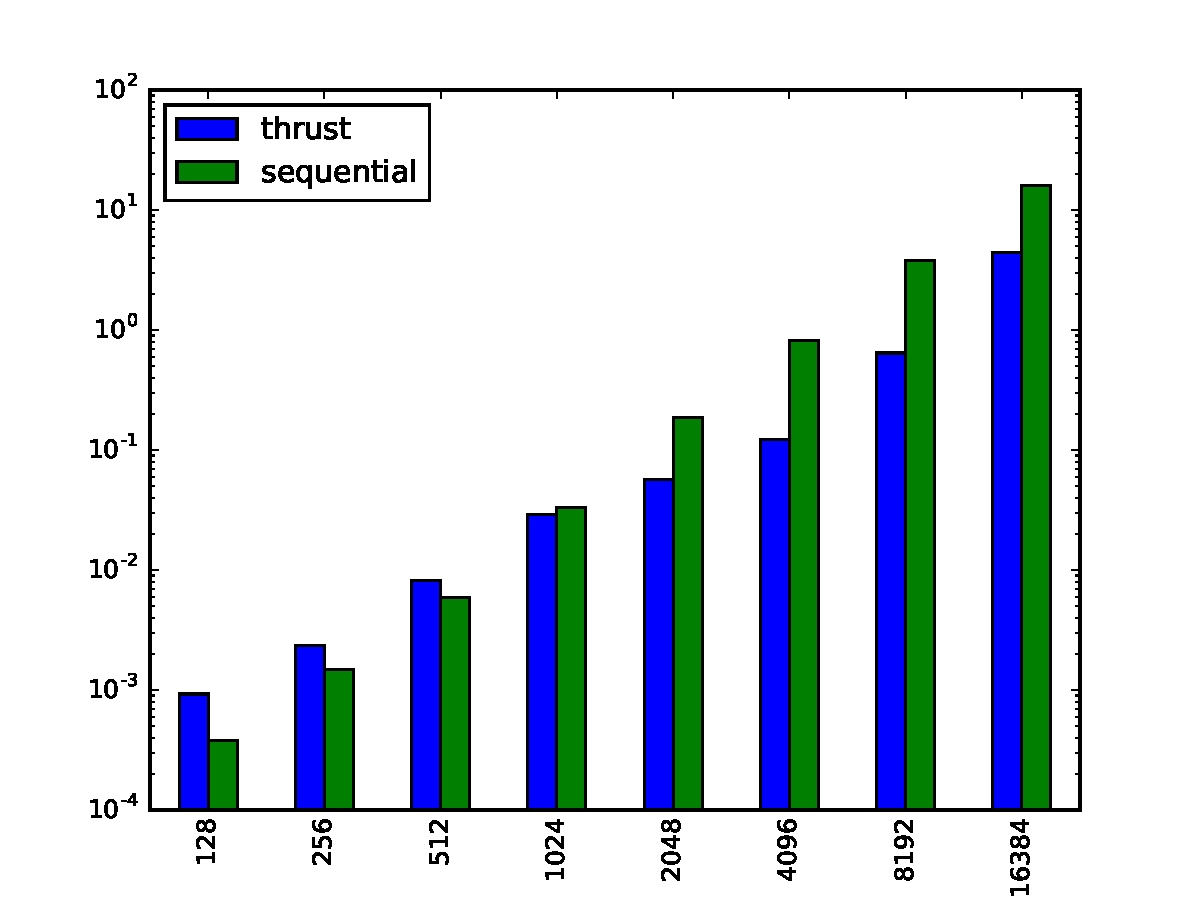
\includegraphics[scale=0.4]{imgs/thrust_vs_sequential_total.pdf} 
    \end{column}
    \begin{column}{3cm}
      \begin{itemize}
        \item code handles horizontal and vertical passes by adjusting
          strides
        \item results do not look very promising
      \end{itemize}
    \end{column}
  \end{columns}
\end{frame} 

\begin{frame}{A closer look}
  \begin{columns}
    \begin{column}{7cm}
      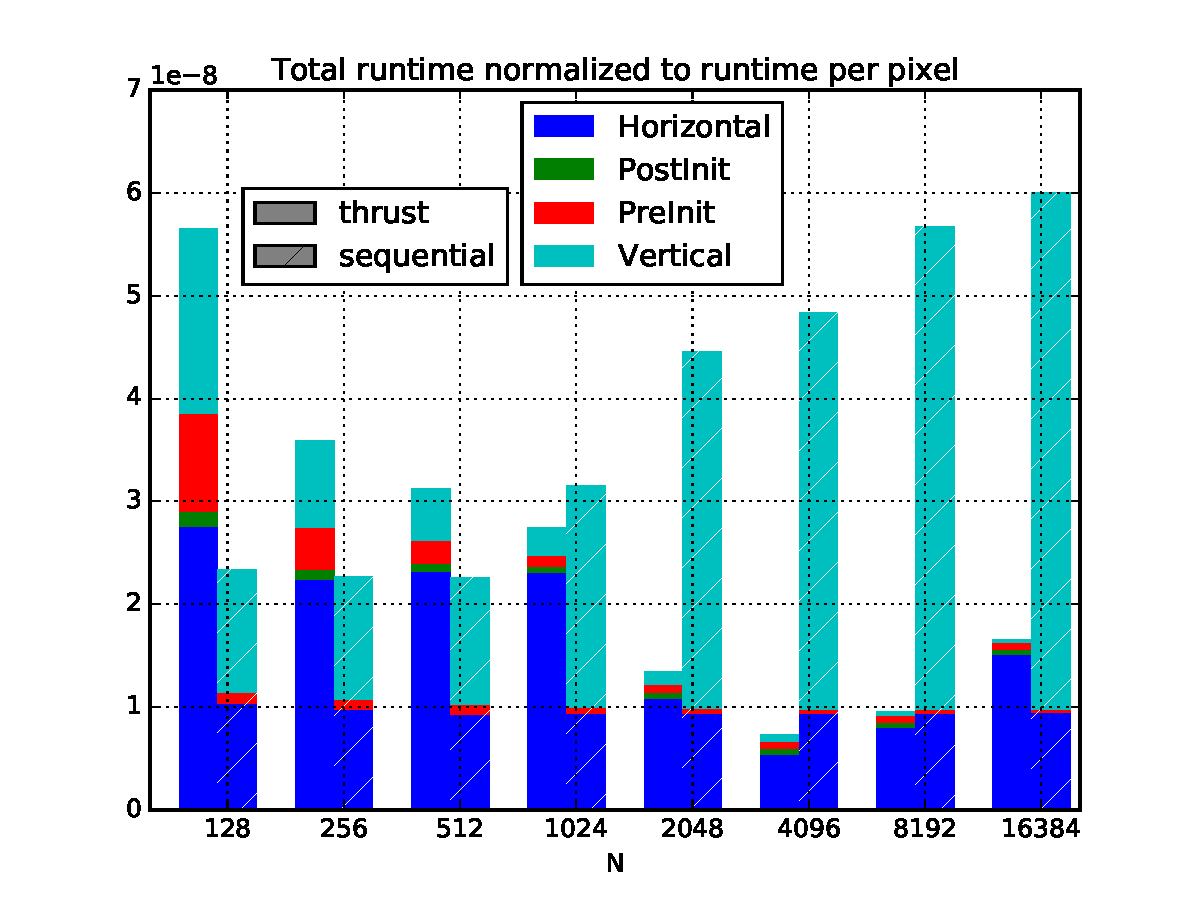
\includegraphics[scale=0.4]{imgs/thrust_vs_sequential_normalized.pdf} 
    \end{column}
    \begin{column}{5cm}
      \begin{itemize}
        \item Initialization and data transfer not limiting
        \item Sequential version's performance degrades for the vertical
          pass - stride causes cache misses
        \item Thrust version is limited by performance of horizontal pass -
          results in non-coalesced memory access (consecutive threads access
          strided data)
      \end{itemize}
    \end{column}
  \end{columns}
\end{frame} 

\subsection{Parallelizing causal and anti-causal pass}
\begin{frame}[fragile]
\frametitle{Streams}
Just run them on two different streams!
  \begin{lstlisting}[basicstyle=\tiny]
thrust::for_each_n(
  thrust::cuda::par.on(stream),
  thrust::counting_iterator<int>(0), height,
  ...
  \end{lstlisting}
  \begin{figure}
      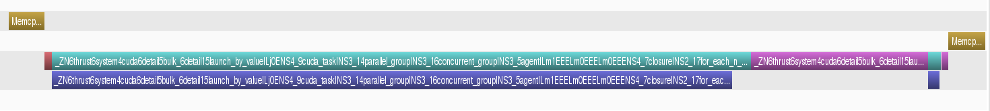
\includegraphics[scale=0.3]{imgs/overlap.png} 
  \end{figure}
  Improves performance but horizontal pass is still the bottleneck.
\end{frame}

\begin{frame}[fragile]
  \frametitle{Reducing causality passes}
  \begin{itemize}
    \item Synchronize streams
    \item Add causal and anticausal buffers into result
  \end{itemize}
  Remember: Anticausal pass goes from right to left - yet the original
  implementation writes into the buffer from left to right:
  \begin{lstlisting}[basicstyle=\tiny]
for(int i = 4; i < width; ++i) {
  row[i * column_stride] =
    c.b_anticausal[1] * src[((width - 1) - i + 1) * column_stride]
  + c.b_anticausal[2] * src[((width - 1) - i + 2) * column_stride]
  + c.b_anticausal[3] * src[((width - 1) - i + 3) * column_stride]
  + c.b_anticausal[4] * src[((width - 1) - i + 4) * column_stride]
  - c.a[1] * row[(i - 1) * column_stride]
  - c.a[2] * row[(i - 2) * column_stride]
  - c.a[3] * row[(i - 3) * column_stride]
  - c.a[4] * row[(i - 4) * column_stride];
}
  \end{lstlisting}
\end{frame}

\begin{frame}[fragile]
  \frametitle{Reducing causality passes}
  $\implies$ need to reverse anticausal buffer in each row:
  \begin{lstlisting}[basicstyle=\tiny]
cudaStreamSynchronize(s1);
cudaStreamSynchronize(s2);
thrust::for_each_n(
  thrust::counting_iterator<int>(0), height,
  [...] __device__ (int n) {
    auto dest = dest_begin + n * row_stride;
    auto row_l = buffer_l_begin + n * row_stride;
    auto row_r = buffer_r_begin + n * row_stride;
    for(int i = 0; i < width; ++i) {
      dest[i * column_stride] =
      row_l[i * column_stride] + row_r[(width - 1 - i) * column_stride];
    }
  });
  \end{lstlisting}
  Instead, write buffer from right to left and perform fully parallel
  summation:
  \begin{lstlisting}[basicstyle=\tiny]
thrust::transform(
  buffer_l_begin, buffer_l_begin + width * height,
  buffer_r_begin,
  dest_begin,
  thrust::plus<T>());
  \end{lstlisting}
\end{frame}

\subsection{Improving memory access patterns}
\begin{frame}[fragile]
  \frametitle{Idea}
  \begin{enumerate}
    \item Transpose
    \item Vertical pass
    \item Transpose
    \item Horizontal pass
  \end{enumerate}
  But:
  \begin{itemize}
    \item Two additional transpose operations which are non-trivial to
      implement efficiently on GPUs
    \item Additional buffer for transpose operation required
  \end{itemize}
\end{frame}

\begin{frame}[fragile]
  \frametitle{Even better}
  \begin{itemize}
    \item Even with a simple thrust implementation this achieves speedups
    \item We can avoid the additional buffer by performing the transposition
      during the addition of the causality buffers ($\implies$ perform
      vertical pass first, i.e. work on mirror image or assume column major
      format)
    \item Exactly this, adding two transposed matrices, is also implemented
      in cublas!
  \end{itemize}
  \begin{lstlisting}[basicstyle=\tiny]
T* buffer_l_ptr  = thrust::raw_pointer_cast(&*buffer_l_begin);
T* buffer_r_ptr  = thrust::raw_pointer_cast(&*buffer_r_begin);
T* dest_ptr = thrust::raw_pointer_cast(&*dest_begin);
T alpha = beta = 1.;
cublasSgeam(
  *handle, CUBLAS_OP_T, CUBLAS_OP_T, height, width,
  &alpha, buffer_l_ptr, width,
  &beta, buffer_r_ptr, width,
  dest_ptr, height);
  \end{lstlisting}
\end{frame}

\begin{frame}{Results - Times}
  \begin{columns}
    \begin{column}{7cm}
      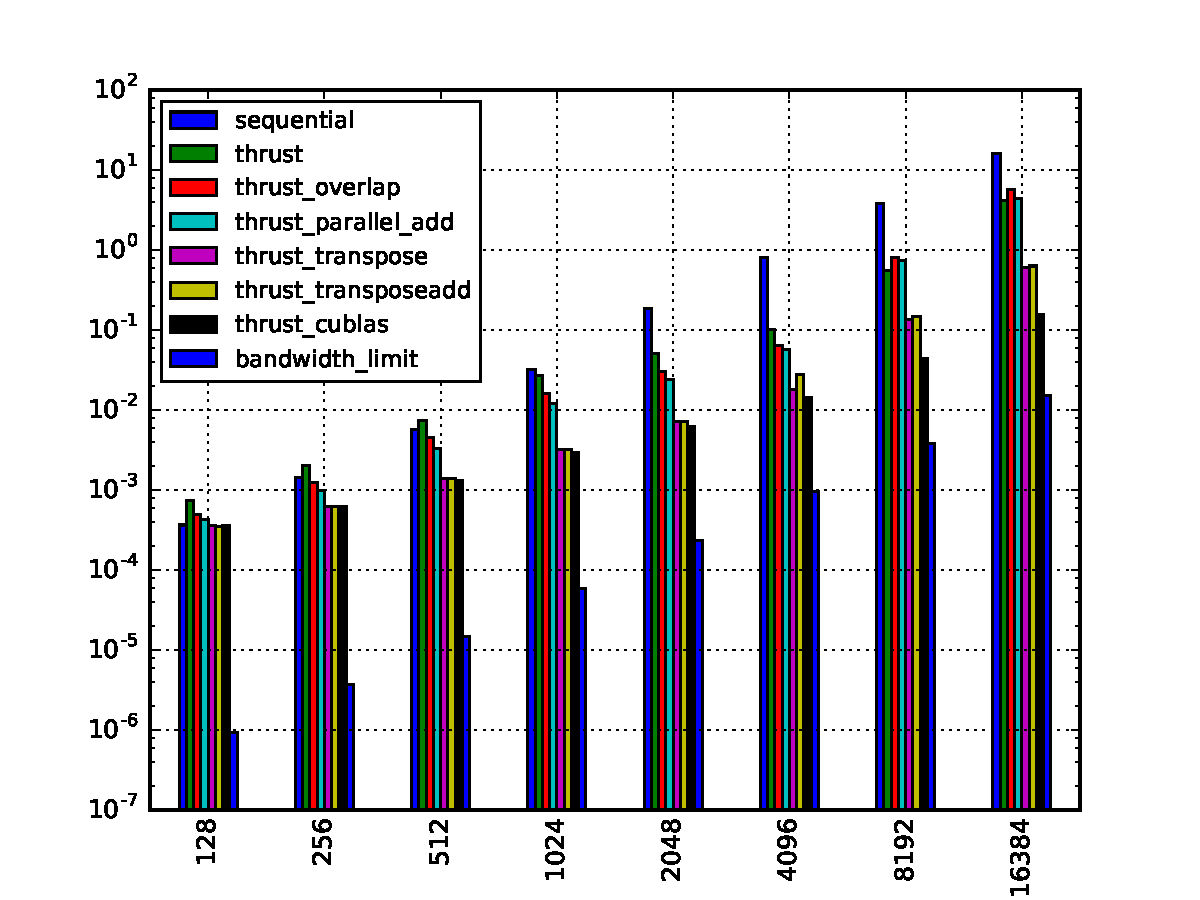
\includegraphics[scale=0.4]{imgs/all_times.pdf} 
    \end{column}
    \begin{column}{3cm}
      \begin{itemize}
        \item Improving memory access most important factor
        \item Optimized cuBLAS geam gives additional boost for larger data
      \end{itemize}
    \end{column}
  \end{columns}
\end{frame} 

\begin{frame}{Results - Speedups}
  \begin{columns}
    \begin{column}{7cm}
      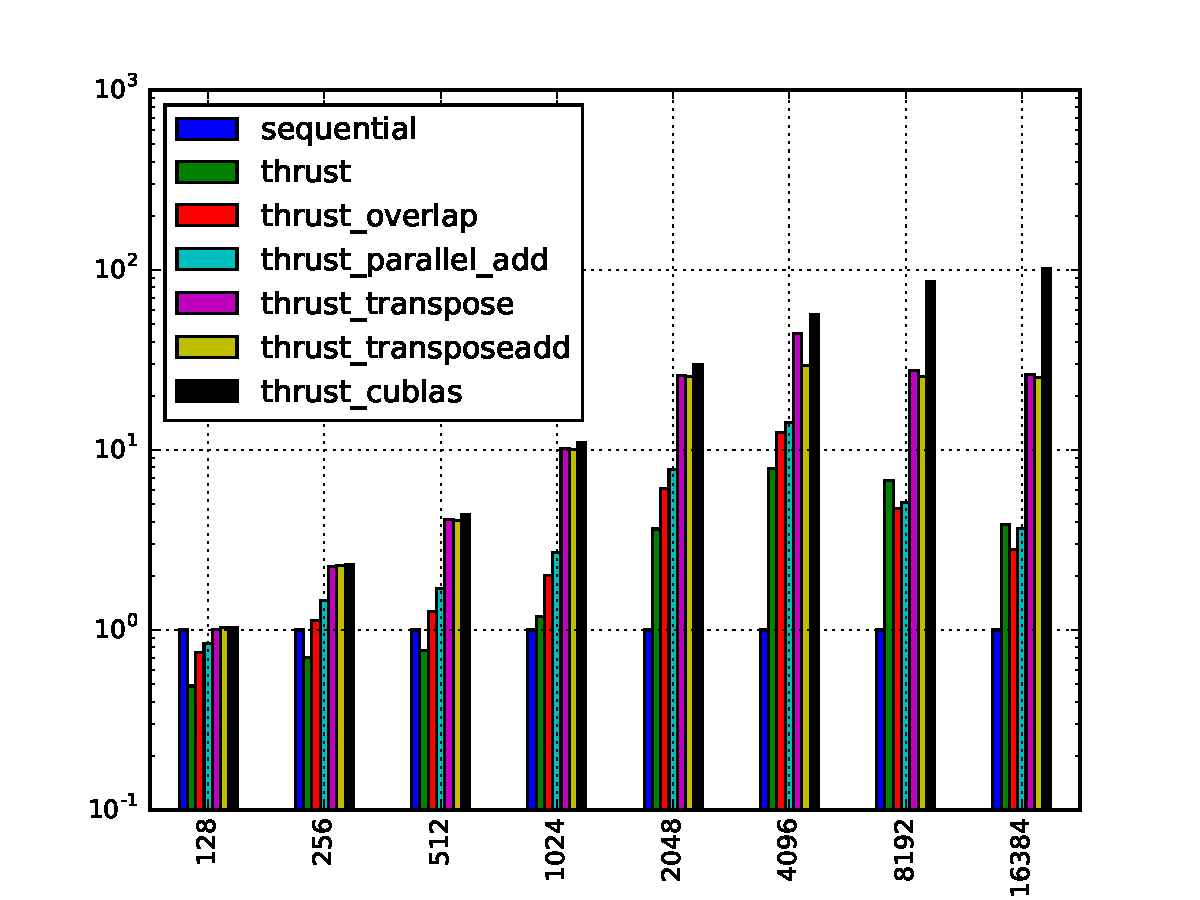
\includegraphics[scale=0.4]{imgs/all_speedups.pdf} 
    \end{column}
    \begin{column}{3cm}
      \begin{itemize}
        \item Maximum speedup of $100$
        \item For $1024x1024$ images: Speedup of $11$ without transfers and $7$ with.
\item $360$ FPS @ $1024x1024$
      \end{itemize}
    \end{column}
  \end{columns}
\end{frame} 

\section{Conclusion} 
\frame{\frametitle{Further considerations}
Different data and applications need different optimizations.
Here: Image sequences of approximately 1024x1024 pixels.
\begin{itemize}
	\item Parallelization of higher order recurrence relations is more complicated (because prefix sum operators are required to be associative for parallelization) \cite{blelloch1990prefix}
	\item It must be evaluated whether a parallelization of the recurrence relation
		within rows pays off for the relatively small number of $1024$ elements.
  \item Multiple features can be calculated concurrently.
  \item Features of multiple images (from a video sequence) can be calculated concurrently.
\end{itemize}
}

\frame{\frametitle{Alternatives}
\begin{itemize}
  \item Evaluate for which parameters FIR and FFT perform better/worse.
  \item Alternative parallelization strategy: blocked parallelism.
\end{itemize}
}

%\begin{frame}[t, allowframebreaks]
\begin{frame}[t]
  \frametitle{References}
  \bibliographystyle{amsalpha}
  \bibliography{doc.bib}
\end{frame}

\end{document}
